\section{Triton Kernel}
\label{appendix:triton}
Given $\mathbf{Q},\mathbf{K},\mathbf{V} \in \mathbb{R}^{b\times h\times n \times n \times d}$ and $\mathbf{B} \in \mathbb{R}^{b\times h\times n \times n}$, where $b$, $h$, and $n$ denote the batch size, number of attention heads, and token length, we implemented a Triton~\cite{tillet2019triton} kernel for the $\mathtt{GatedLinearTriangularAttention}$ module:
\begin{align}
\mathbf{O} &= \left(\left(\mathbf{Q}\mathbf{K}^{T}\right)\odot\mathbf{B}\right)\mathbf{V}
\end{align}
Its gradient can be computed by:
\begin{align}
\mathrm{d}\mathbf{V}&=\left(\left(\mathbf{Q}\mathbf{K}^{T}\right)\odot\mathbf{B}\right)^T\cdot\mathrm{d}\mathbf{O} \\
\mathrm{d}\mathbf{Q}&=\left(\left(\mathrm{d}\mathbf{O}\cdot\mathbf{V}^T\right)\odot\mathbf{B}\right)\cdot\mathbf{K} \\
\mathrm{d}\mathbf{K}&=\left(\left(\mathrm{d}\mathbf{O}\cdot\mathbf{V}^T\right)\odot\mathbf{B}\right)^T\cdot\mathbf{Q} \\
\mathrm{d}\mathbf{B}&=\left(\mathrm{d}\mathbf{O}\cdot\mathbf{V}^T\right)\odot\left(\mathbf{Q}\mathbf{K}^T\right)
\end{align}
Notably, the same kernel can be used for computing $\mathbf{O}$, $\mathrm{d}\mathbf{Q}$, $\mathrm{d}\mathbf{K}$, and $\mathrm{d}\mathbf{V}$, whereas $\mathrm{d}\mathbf{B}$ can be implemented through two blocked matrix multiplications. Figure~\ref{fig:triton} illustrates the implementation of this kernel. We treat the $b\times h$ dimensions as a single batch dimension and parallelize over the first dimension of size $n$. Within each process, we iterate over the second dimension of size $n$ to aggregate the result, thereby avoiding the materialization of the full $n\times n$ matrix.

\begin{figure}[h]
    \centering
    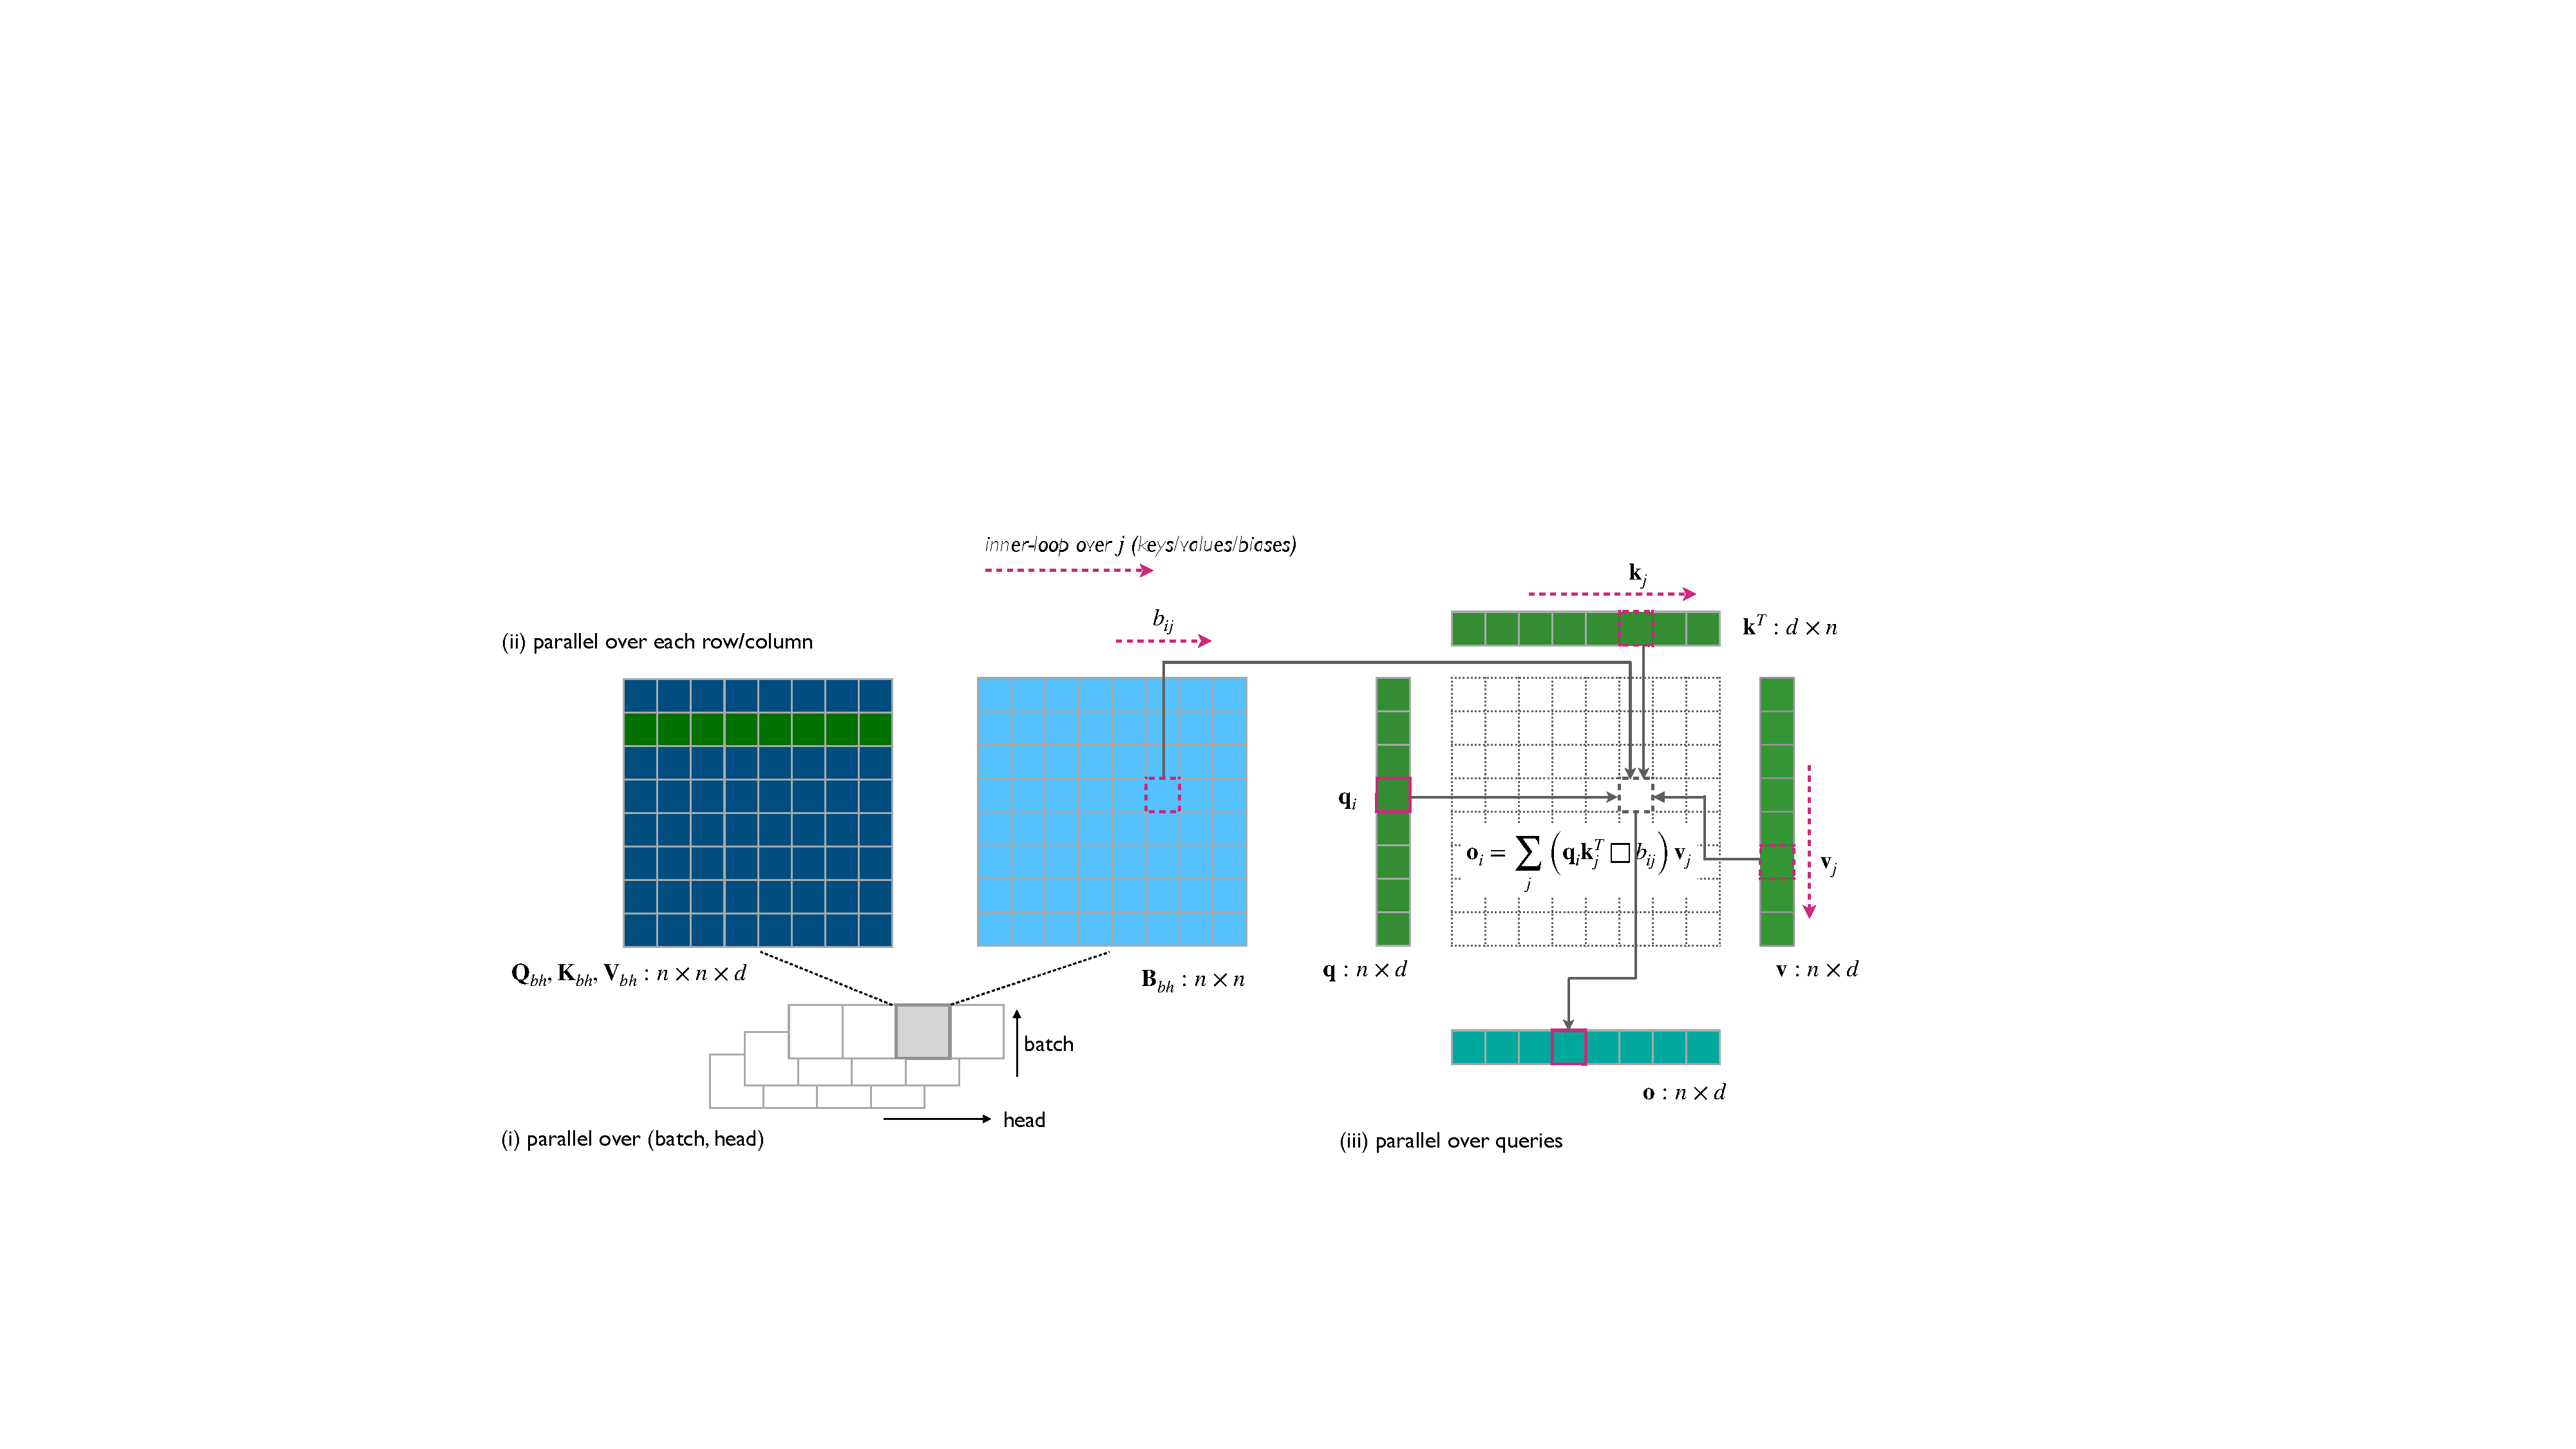
\includegraphics[width=1.0\linewidth]{figures/triton.pdf}
    \caption{The Triton implementation of \texttt{LinearTriangularAttention}.}
    \label{fig:triton}
\end{figure}


\section{Datasets}
\label{appendix:data}

% \subsection{Experimental Dataset} 
% We closely followed the preprocessing steps of AlphaFold 3, 

% \subsection{Distillation Dataset} 
We plot the probability density distribution of the protein lengths in the AFDB dataset and the MGnify dataset in Figure~\ref{fig:data_length_dist}. The length distribution of AFDB is skewed toward short proteins, with a median length of $95$, whereas the length distribution of MGnify is more uniform. 

\begin{figure}[h]
    \centering
    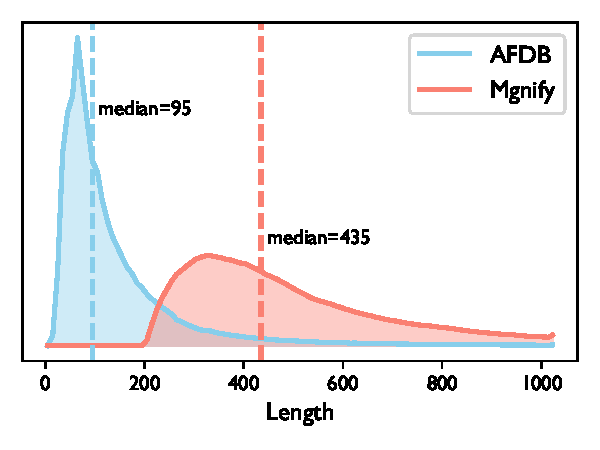
\includegraphics[width=0.4\linewidth]{figures/data_length_dist.pdf}
    \caption{The probability density distribution of sequence lengths for different datasets. The AFDB dataset is dominated by short sequences, while MGnify contains more long sequences.}
    \label{fig:data_length_dist}
\end{figure}

\begin{figure}[h]
    \centering
    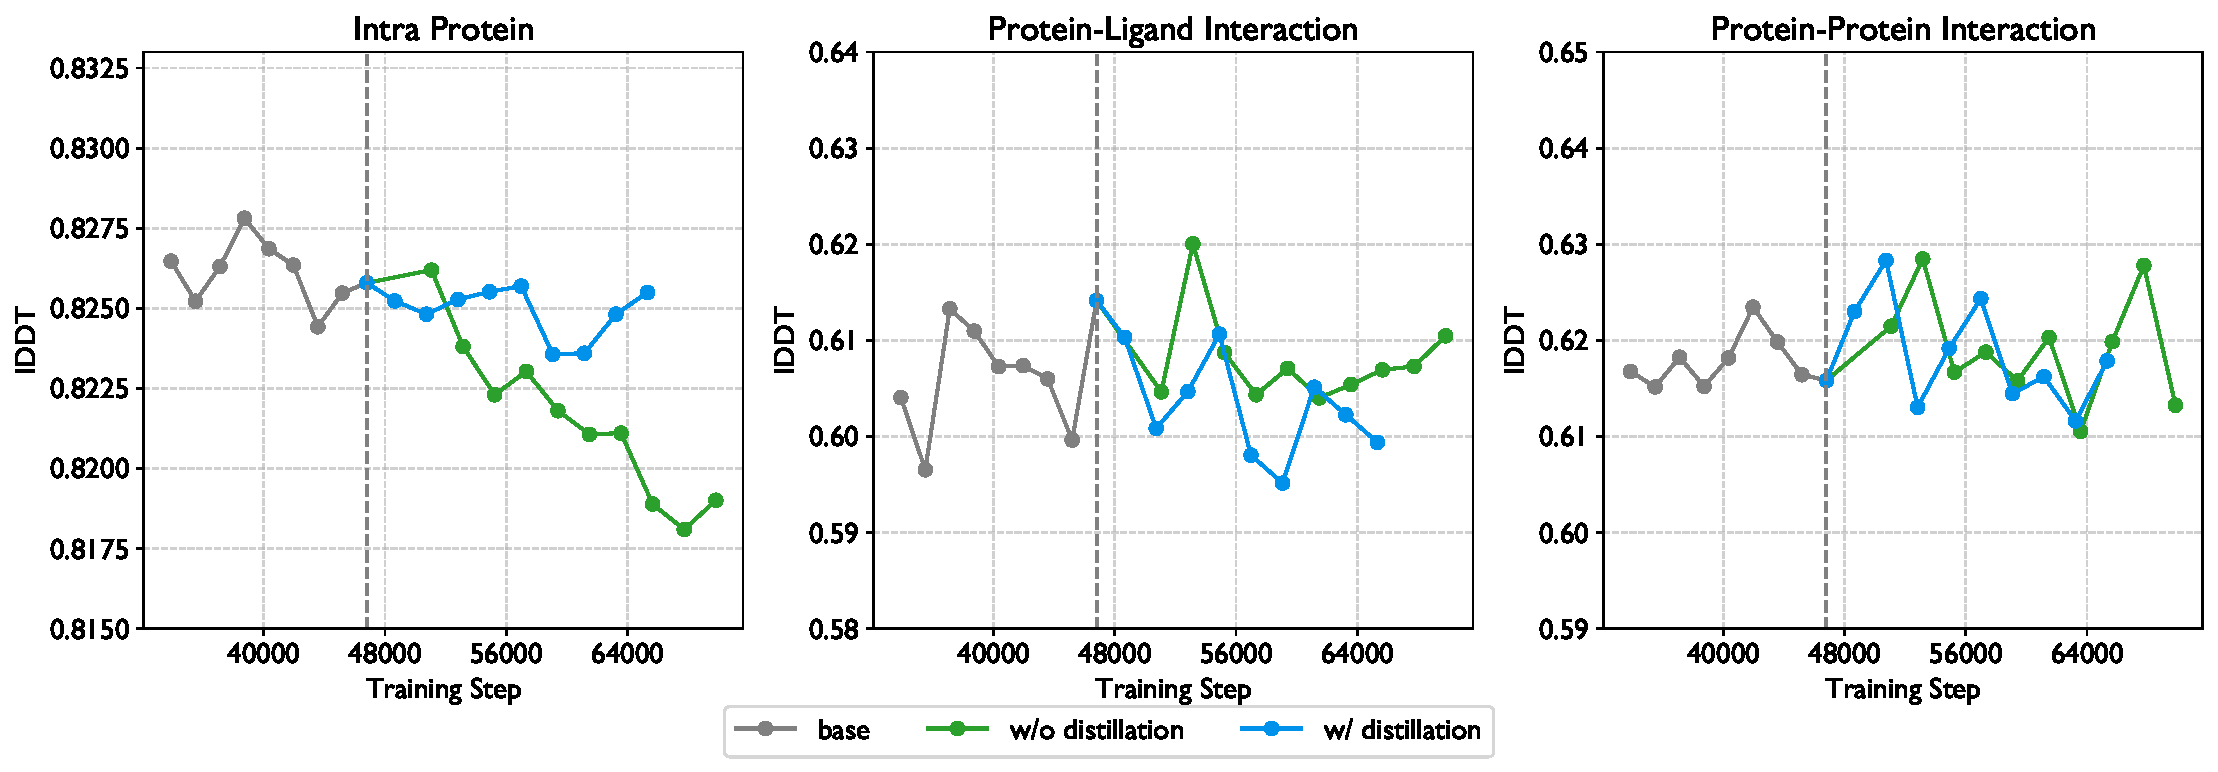
\includegraphics[width=1.0\linewidth]{figures/distill.pdf}
    \caption{The effect of removing distillation data at certain stages. The grey curve represents the base model from which the continual training stage initiates. The green and blue curves denote the model trained with and without distillation data, respectively. Removal of distillation data leads to a significant degradation in intra-protein lDDT.}
    \label{fig:distill}
\end{figure}


\section{Training Stability during Scaling}
\label{appendix:scaling_stability}


Scaling model capacity introduced several training stability issues. This section documents the challenges and our solutions. As the model size increases, we observed gradient explosion issues, particularly in the early stages of training. To address this, we applied gradient clipping and adjusted the learning rate schedule.


% \paragraph{Gradient Explosion}

\begin{itemize}
    \item \textbf{Learning Rate Adjustment}: When scaling from Medium ($256$-width) to Large ($512$-width), we found it necessary to reduce the learning rate and adjust optimization hyperparameters to stabilize training.
    \item \textbf{Warm-up Strategy}: We employed an extended warm-up period from $1000$ to $3000$ for larger models to ensure stable convergence in the initial training phase.
\end{itemize}
% \paragraph{Learning Rate Adjustment}
% \paragraph{Warm-up Strategy}

We denote the original Large model without stability optimization (smaller learning rate with longer warmup steps) as \texttt{Large-Raw}, and the optimized version as \texttt{Large}. Figure~\ref{fig:scaling_stability_training} illustrates the training dynamics during the early $5000$ steps. The \texttt{Large-Raw} model exhibits unstable training behavior with significant loss fluctuations, while the \texttt{Large} model with optimized hyperparameters demonstrates stable convergence. Figure~\ref{fig:scaling_stability_validation} presents the validation metrics comparison, showing that the stability optimization not only improves training dynamics but also leads to better final performance.

\begin{figure}[!htbp]
    \centering
    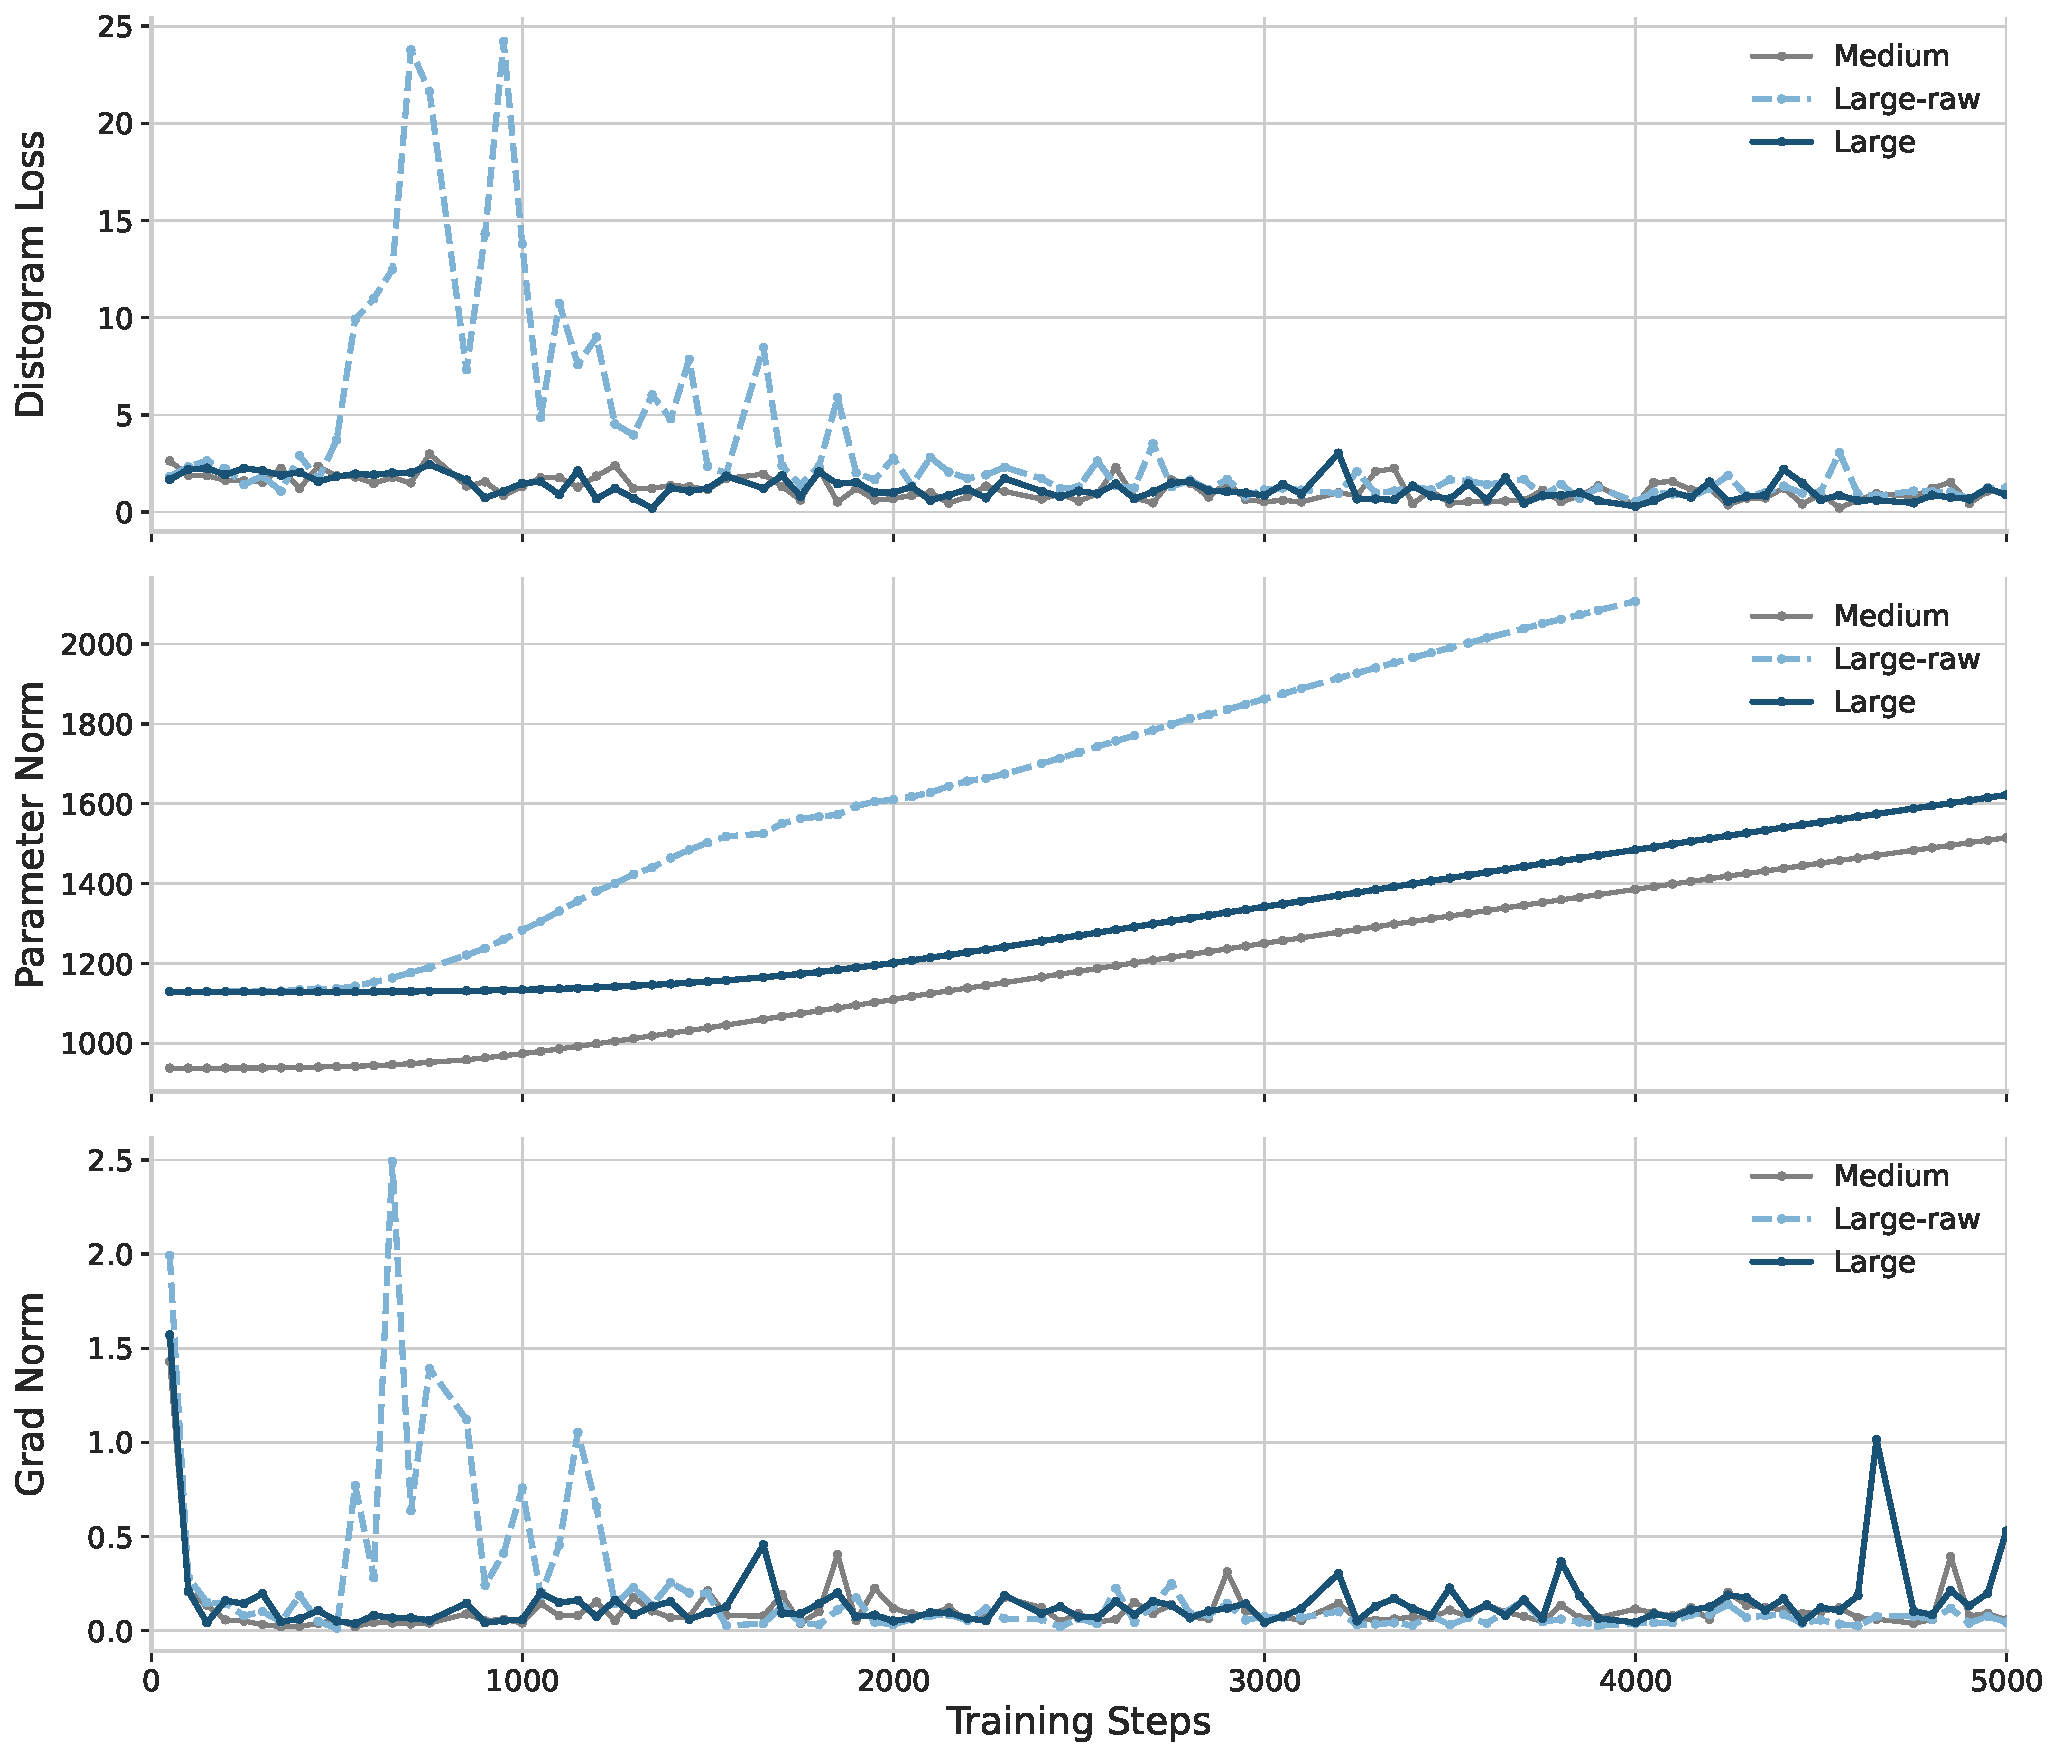
\includegraphics[width=0.8\linewidth]{figures/scaling_stability_training_early_5000steps.pdf}
    \caption{Training dynamics during the early $5000$ steps. The \texttt{Large-Raw} model shows unstable training with loss spikes, while the \texttt{Large} model with optimized hyperparameters exhibits stable convergence.}
    \label{fig:scaling_stability_training}
\end{figure}

\begin{figure}[!htbp]
    \centering
    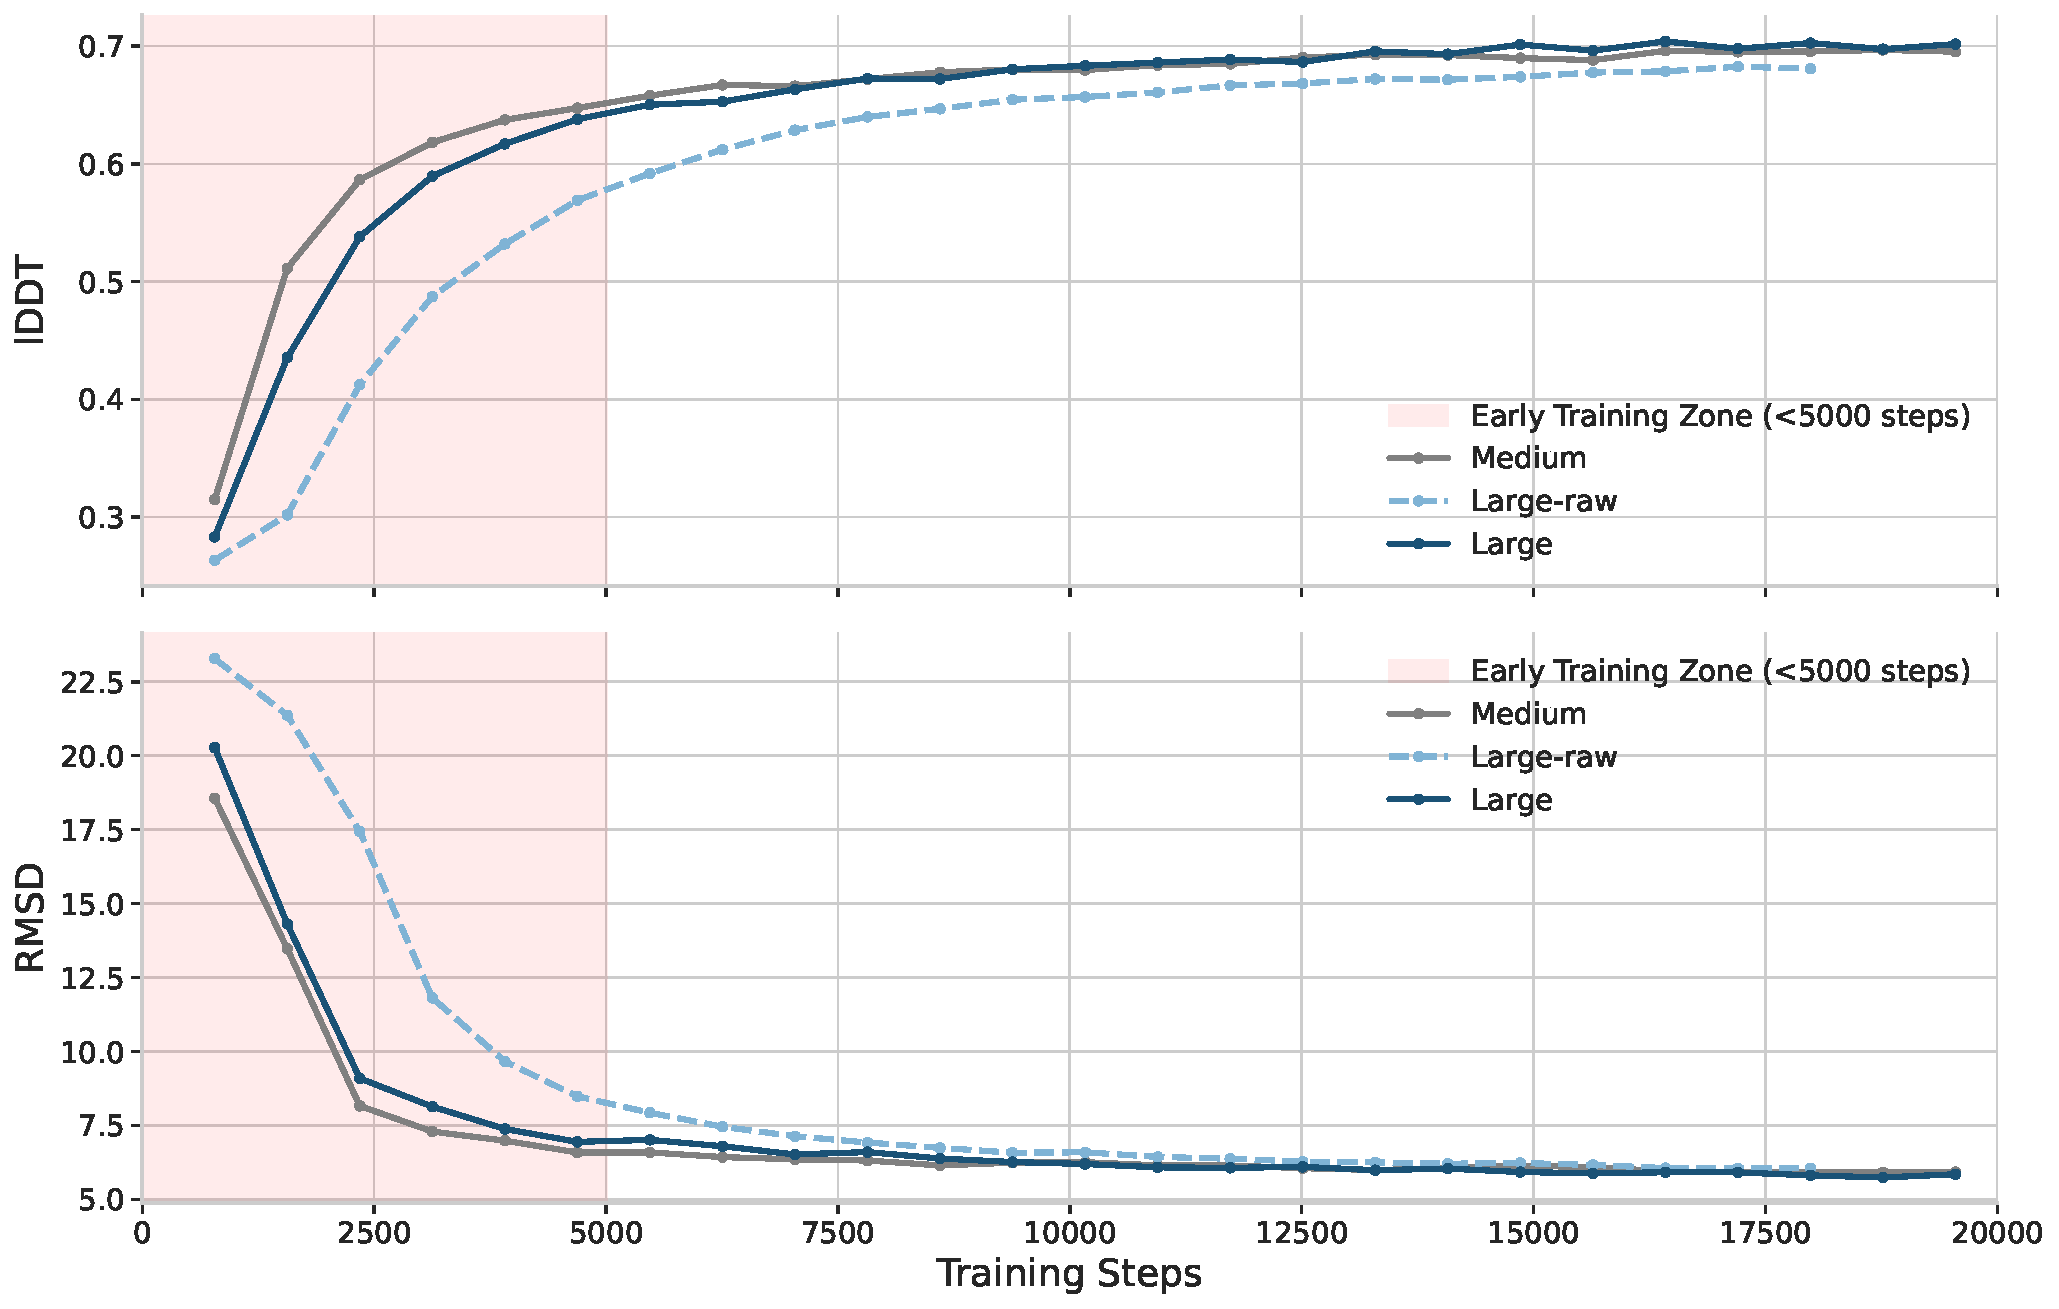
\includegraphics[width=0.8\linewidth]{figures/scaling_stability_validation_metrics.pdf}
    \caption{Validation metrics comparison between \texttt{Large-Raw} and \texttt{Large}. The stability optimization leads to improved performance across validation metrics.}
    \label{fig:scaling_stability_validation}
\end{figure}

\section{Design Space of Linear Triangular Attention}

Although modern linear attention has been thoroughly studied in autoregressive language models~\cite{kimiteam2025kimilinearexpressiveefficient,minimax2025minimax01scalingfoundationmodels}, it remains an open question as to how one should incorporate the bias term into non-autoregressive linear attention, i.e., linear triangular attention. This section briefly discusses the design space of linear triangular attention. 
% and (ii) methods to stabilize the training process. 

Despite the simplicity of the mathematical formulation of linear attention, several design choices remain to be determined in practical implementation. We start with the basic form, $\phi(\mathbf{Q}_i)\phi(\mathbf{K}_i^T)\mathbf{V}_i$, where $\mathbf{Q}_i, \mathbf{K}_i, \mathbf{V}_i\in\mathbf{R}^{n\times d}$ are the $i$-th row of the queries, keys, and values. The first question is how to bound the values of output feature vectors to prevent the explosion or vanishing of hidden states. A simple yet effective choice is to normalize the attention score with their summation, similar to the \texttt{softmax} attention:
\begin{align}
\frac{\left[\phi(\mathbf{Q}_i)\phi(\mathbf{K}_i^T)\Box\psi(\mathbf{B})\right]\mathbf{V}_i}{\left[\phi(\mathbf{Q}_i)\phi(\mathbf{K}_i^T)\Box\psi(\mathbf{B})\right]\mathbf{1}^{n\times 1}},
\end{align}
where $\mathbf{B}\in\mathbb{R}^{n\times n}$, and $\Box$ can be an arbitrary operation. Such a formulation has proven its effectiveness in modern generative tasks, such as ViT-based high-resolution image synthesis~\cite{xie2023efficient,xie2024sana}. However, there is a potential risk for applying this architecture: if we want to introduce a bias term into the formulation, we still have to materialize a $n\times n$ matrix in the denominator, which is memory-intensive. Besides, a challenge of training linear attention in this form is that the unbounded gradients may lead to unstable convergence~\cite{qin2022devil}. We adopt an alternative approach proposed in Lightning Attention~\cite{qin2024lightning}: dropping the normalization term in the denominator while applying a \texttt{LayerNorm} layer to the output:
\begin{align}
\mathtt{LayerNorm}_{\texttt{over-head/hidden}}\left(\left[\phi(\mathbf{Q}_i)\phi(\mathbf{K}_i^T)\Box\psi(\mathbf{B})\right]\mathbf{V}_i\right).
\end{align}
In the above formulation, there are two final options to be determined: (i) how to select the feature function $\phi$, and (ii) whether to apply the normalization layer to the hidden dimension or the head dimension. Through comprehensive ablation studies, we found that the original configuration ($\phi=\mathtt{silu}$, $\texttt{LayerNormOverHead}$) in Lightning Attention~\cite{qin2024lightning} failed to converge in folding tasks, so we switched to ($\phi=\mathtt{relu}$, $\texttt{LayerNormOverHidden}$), which enabled us to achieve substantially better performance. In Figure~\ref{fig:linatt_choices}, we employ the distogram loss as an indicator to evaluate how well the module fits the data. 

\begin{figure}[h]
    \centering
    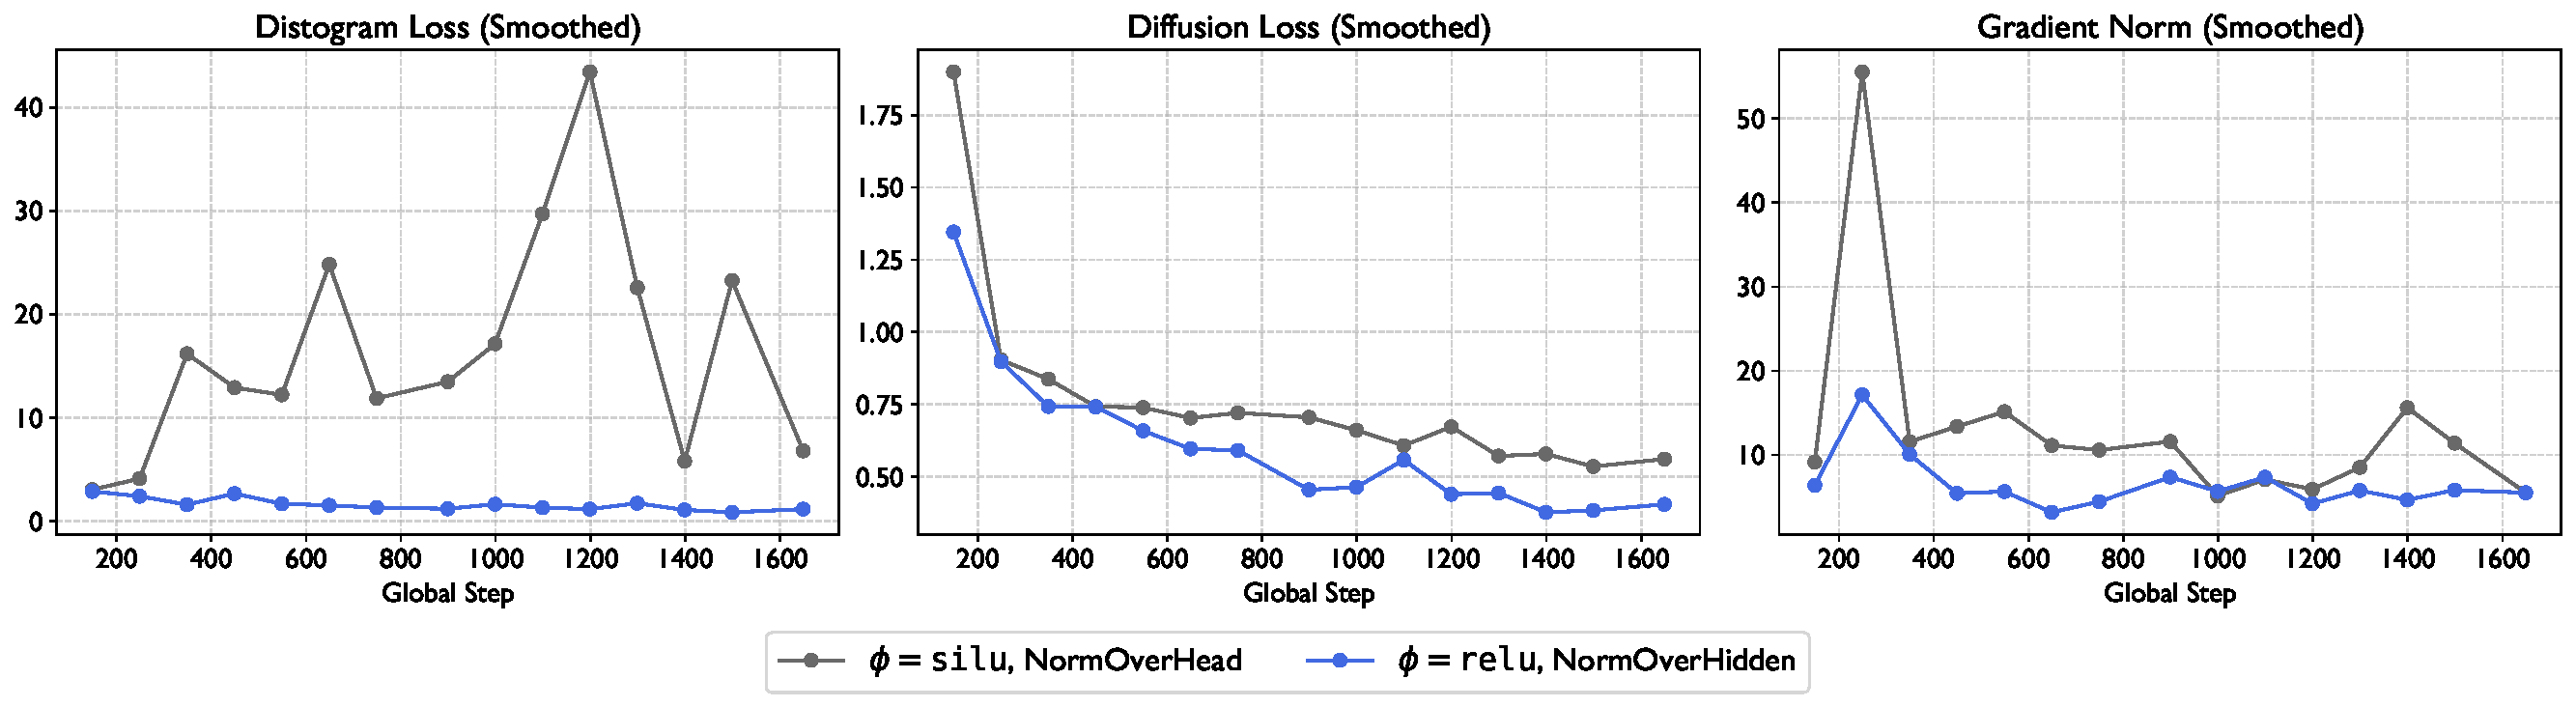
\includegraphics[width=1.0\linewidth]{figures/linatt_choices.pdf}
    \caption{Our choice of feature function and the normalization strategy stablizes the training process, while the original version fails to converge. The distogram loss serves as a direct signal to indicate the convergence.}
    \label{fig:linatt_choices}
\end{figure}

% \paragraph{Scaling Stability} Despite its advantages in spatial and temporal efficiency, linear attention is less favored than its counterpart, standard softmax attention. Some early work points out that the linearization of attention tends to reduce the rank of the output feature vectors, thereby diminishing the capacity of the module~\cite{fan2025breaking}. Such performance degradation can be partially mitigated by scaling the model size, i.e., increasing the dimension of the $\mathbf{K}^T\mathbf{V}$'s state space. However, as the hidden size increases, the training dynamics of linear attention become unstable. We found that increasing the number of warmup steps (from $1000$ to $3000$) was essential such that the adaptive optimizer can better approximate the momentum statistics of the gradients~\cite{liu2019variance}.

\section{Comparison of Two Linear Attention}

\begin{figure}[h]
    \centering
    \begin{minipage}[t]{0.32\textwidth}
        \centering
        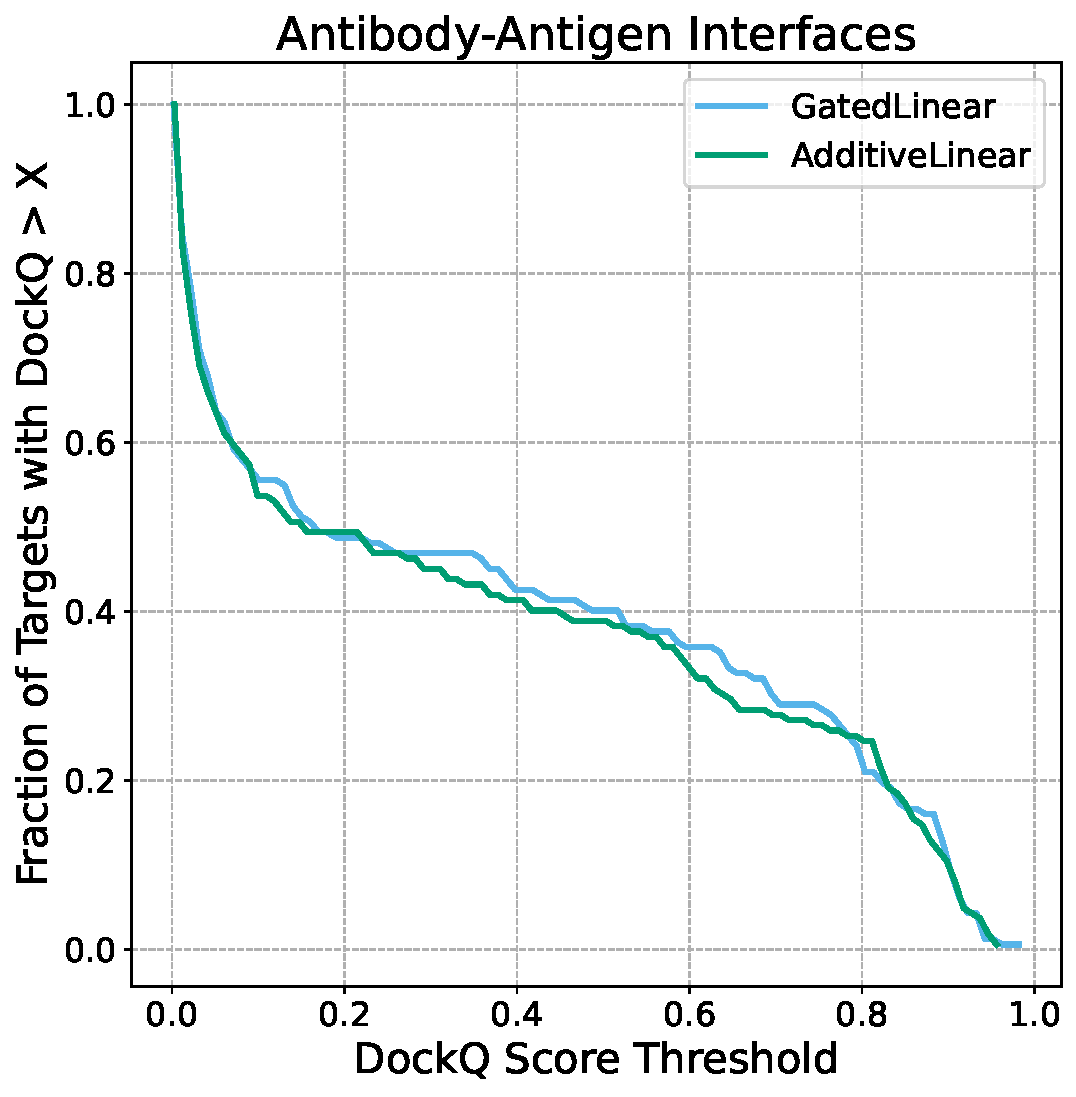
\includegraphics[width=\linewidth]{figures/lin_interface_antibody_antigen_cumulative_dockq.pdf}
        % (a) Ab-Ag
    \end{minipage}
    \hfill
    \begin{minipage}[t]{0.32\textwidth}
        \centering
        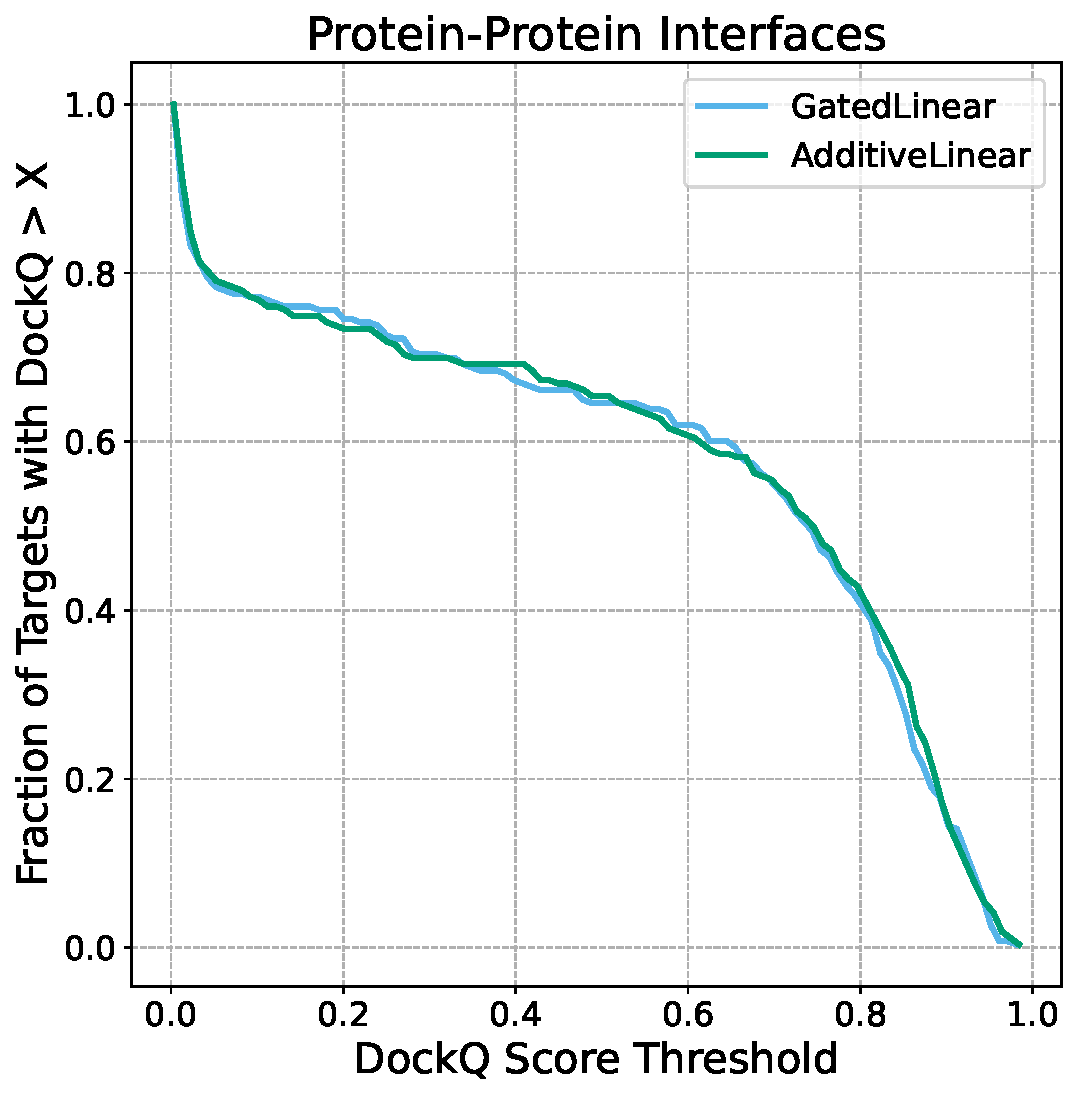
\includegraphics[width=\linewidth]{figures/lin_interface_protein_protein_cumulative_dockq.pdf}
        % (b) Protein-Protein 
    \end{minipage}
    \hfill
    \begin{minipage}[t]{0.32\textwidth}
        \centering
        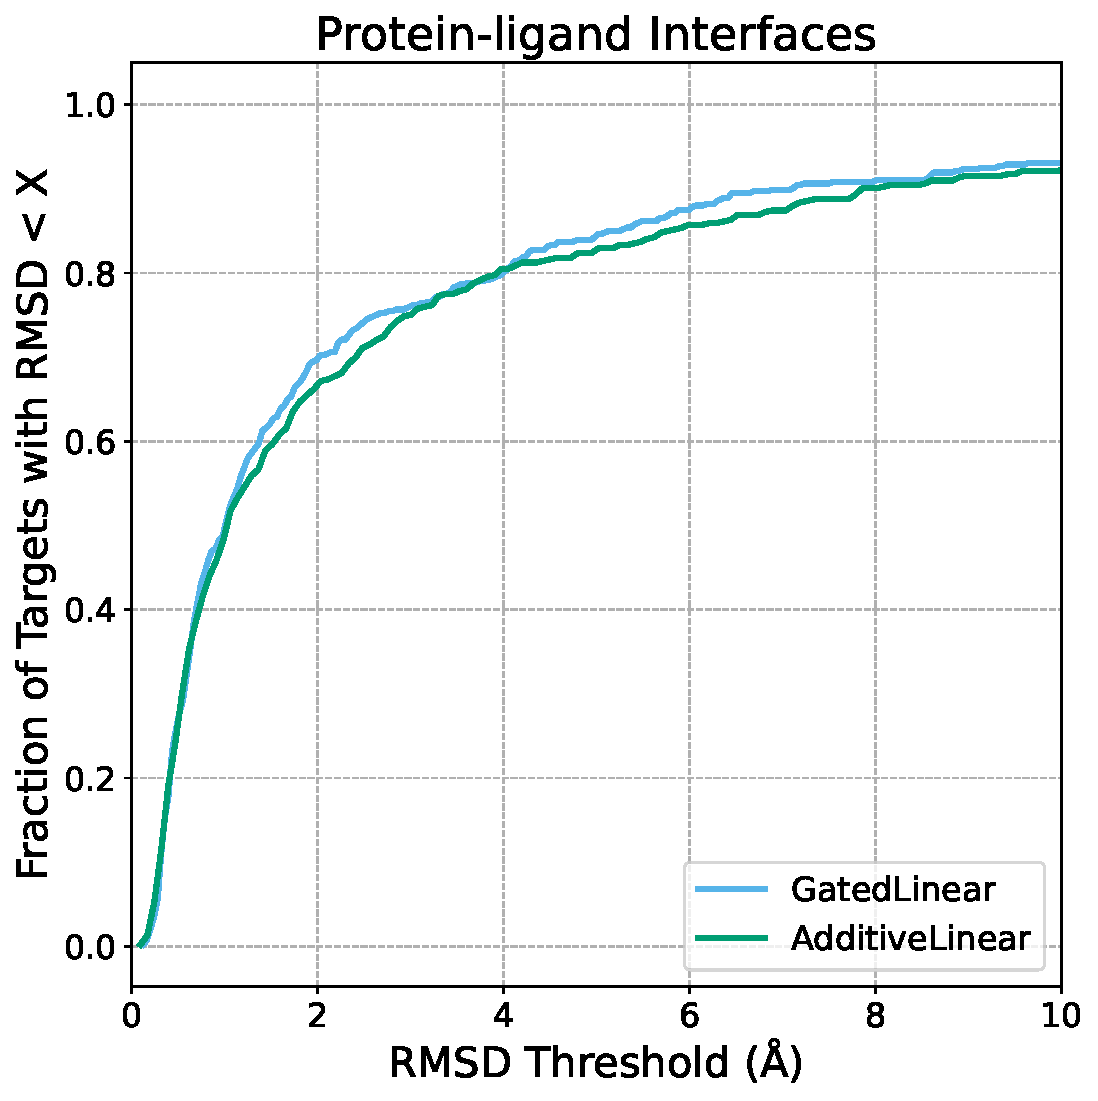
\includegraphics[width=\linewidth]{figures/lin_interface_protein_ligand_cumulative_rmsd.pdf}
        % (c) Protein-Ligand
    \end{minipage}
    \caption{Cumulative distribution of interface prediction success rates across different modalities for linear attention based models. We find that \texttt{GatedLinearTriAtt} slightly outperforms the \texttt{AdditiveLinearTriAtt} module on antibody-antigen and protein-ligand interaction. Therefore, we finally chose \texttt{GatedLinearTriAtt} as the default attention configuration.}
    \label{fig:lin_interface_distribution}
\end{figure}